\begin{frame}{}
\begin{columns}
    \begin{column}{0.8\textwidth}
        \begin{heading}{Symbols}
            \begin{itemize}
                \item \(B=\set{b_1,b_2,b_3}\) - last independent set in path \(i\)
                \item \(A=\set{a_1,a_2,a_3}\) - first independent set in path \(i+1\)
                \item \(b_1\) - last vertex modified to obtain \(B\) in path \(i\)
                \item \(a_3\) - first vertex modified in path \(i+1\)
            \end{itemize}
        \end{heading}
        \onslide<2->{
        \begin{heading}{Construction}
        \begin{itemize}
            \item we add \(3k-2\) new vertices \(x_i\) and connect them with everything
            \onslide<3->{
            \item remove vertices \((x_i,\ x_j)\) for \(|i-j|<k\)
            }
            \onslide<4->{
            \item remove vertices \((x_i,b_j)\), \((x_{3k-2-i}, a_{k-j})\) for \(j>i\)
            }
        \end{itemize}
        \end{heading}
        }
    \end{column}
    \begin{column}{0.3\textwidth}
        \begin{figure}
            \centering
            \begin{tikzpicture}[scale=0.85]
\coordinate (a0) at (2,0);
\coordinate (a1) at (1,0);
\coordinate (a2) at (0,0);

\coordinate (b0) at (2,8);
\coordinate (b1) at (1,8);
\coordinate (b2) at (0,8);

\coordinate (x1) at (3,1);
\coordinate (x2) at (3,2);
\coordinate (x3) at (3,3);
\coordinate (x4) at (3,4);
\coordinate (x5) at (3,5);
\coordinate (x6) at (3,6);
\coordinate (x7) at (3,7);
\coordinate (x8) at (3,8);

\draw[line width=1.5pt, dashed] (a0) to (a1);
\draw[line width=1.5pt, dashed] (a1) to (a2);
\draw[line width=1.5pt, bend left=90, dashed] (a0) to (a2);

\draw[line width=1.5pt, dashed] (b0) to (b1);
\draw[line width=1.5pt, dashed] (b1) to (b2);
\draw[line width=1.5pt, bend right=90, dashed] (b0) to (b2);

\only<3->{
    \draw[line width=1.5pt, dashed] (x1) to (x2);
    \draw[line width=1.5pt, dashed] (x2) to (x3);
    \draw[line width=1.5pt, dashed] (x3) to (x4);
    \draw[line width=1.5pt, dashed] (x4) to (x5);
    \draw[line width=1.5pt, dashed] (x5) to (x6);
    \draw[line width=1.5pt, dashed] (x6) to (x7);

    \draw[line width=1.5pt, bend right=90, dashed] (x1) to (x3);
    \draw[line width=1.5pt, bend left=90, dashed] (x2) to (x4);
    \draw[line width=1.5pt, bend right=90, dashed] (x3) to (x5);
    \draw[line width=1.5pt, bend left=90, dashed] (x4) to (x6);
    \draw[line width=1.5pt, bend right=90, dashed] (x5) to (x7);
}
\only<4->{
    \draw[line width=1.5pt, dashed] (a0) to (x1);
    \draw[line width=1.5pt, bend left=40, dashed] (a0) to (x2);
    \draw[line width=1.5pt, bend left=30, dashed] (a1) to (x1);

    \draw[line width=1.5pt, dashed] (b0) to (x7);
    \draw[line width=1.5pt, bend right=40, dashed] (b0) to (x6);
    \draw[line width=1.5pt, bend right=30,dashed] (b1) to (x7);
}

\only<1>{
    \node[circle, draw=black, fill=white, line width=1.5pt, font=\footnotesize] at (a2)  {$a_{3}$};
    \node[circle, draw=black, fill=white, line width=1.5pt, font=\footnotesize] at (a1) {$a_{2}$};
    \node[circle, draw=black, fill=white, line width=1.5pt, font=\footnotesize] at (a0)  {$a_{1}$};

    \node[circle, draw=black, fill=white, line width=1.5pt, font=\footnotesize] at (b2) {$b_1$};
    \node[circle, draw=black, fill=white, line width=1.5pt, font=\footnotesize] at (b1) {$b_2$};
    \node[circle, draw=black, fill=white, line width=1.5pt, font=\footnotesize] at (b0) {$b_3$};
}

\only<2-4>{
    \node[circle, draw=black, fill=white, line width=1.5pt, font=\footnotesize] at (a2)  {$a_{3}$};
    \node[circle, draw=black, fill=white, line width=1.5pt, font=\footnotesize] at (a1) {$a_{2}$};
    \node[circle, draw=black, fill=white, line width=1.5pt, font=\footnotesize] at (a0)  {$a_{1}$};

    \node[circle, draw=black, fill=white, line width=1.5pt, font=\footnotesize] at (b2) {$b_1$};
    \node[circle, draw=black, fill=white, line width=1.5pt, font=\footnotesize] at (b1) {$b_2$};
    \node[circle, draw=black, fill=white, line width=1.5pt, font=\footnotesize] at (b0) {$b_3$};
    
    \node[circle, draw=black, fill=white, line width=1.5pt, font=\footnotesize] at (x1) {$x_{7}$};
    \node[circle, draw=black, fill=white, line width=1.5pt, font=\footnotesize] at (x2) {$x_{6}$};
    \node[circle, draw=black, fill=white, line width=1.5pt, font=\footnotesize] at (x3) {$x_{5}$};
    \node[circle, draw=black, fill=white, line width=1.5pt, font=\footnotesize] at (x4) {$x_{4}$};
    \node[circle, draw=black, fill=white, line width=1.5pt, font=\footnotesize] at (x5) {$x_{3}$};
    \node[circle, draw=black, fill=white, line width=1.5pt, font=\footnotesize] at (x6) {$x_{2}$};
    \node[circle, draw=black, fill=white, line width=1.5pt, font=\footnotesize] at (x7) {$x_{1}$};
}

\only<5>{
    \node[circle, draw=black, fill=white, line width=1.5pt, font=\footnotesize] at (a2)  {$a_{3}$};
    \node[circle, draw=black, fill=white, line width=1.5pt, font=\footnotesize] at (a1) {$a_{2}$};
    \node[circle, draw=black, fill=white, line width=1.5pt, font=\footnotesize] at (a0)  {$a_{1}$};

    \node[circle, draw=black, fill=cfred, line width=1.5pt, font=\footnotesize] at (b2) {$b_1$};
    \node[circle, draw=black, fill=cfred, line width=1.5pt, font=\footnotesize] at (b1) {$b_2$};
    \node[circle, draw=black, fill=cfred, line width=1.5pt, font=\footnotesize] at (b0) {$b_3$};
    
    \node[circle, draw=black, fill=white, line width=1.5pt, font=\footnotesize] at (x1) {$x_{7}$};
    \node[circle, draw=black, fill=white, line width=1.5pt, font=\footnotesize] at (x2) {$x_{6}$};
    \node[circle, draw=black, fill=white, line width=1.5pt, font=\footnotesize] at (x3) {$x_{5}$};
    \node[circle, draw=black, fill=white, line width=1.5pt, font=\footnotesize] at (x4) {$x_{4}$};
    \node[circle, draw=black, fill=white, line width=1.5pt, font=\footnotesize] at (x5) {$x_{3}$};
    \node[circle, draw=black, fill=white, line width=1.5pt, font=\footnotesize] at (x6) {$x_{2}$};
    \node[circle, draw=black, fill=white, line width=1.5pt, font=\footnotesize] at (x7) {$x_{1}$};
}

\only<6>{
    \node[circle, draw=black, fill=white, line width=1.5pt, font=\footnotesize] at (a2)  {$a_{3}$};
    \node[circle, draw=black, fill=white, line width=1.5pt, font=\footnotesize] at (a1) {$a_{2}$};
    \node[circle, draw=black, fill=white, line width=1.5pt, font=\footnotesize] at (a0)  {$a_{1}$};

    \node[circle, draw=black, fill=cfred!20, line width=1.5pt, font=\footnotesize] at (b2) {$b_1$};
    \node[circle, draw=black, fill=cfred, line width=1.5pt, font=\footnotesize] at (b1) {$b_2$};
    \node[circle, draw=black, fill=cfred, line width=1.5pt, font=\footnotesize] at (b0) {$b_3$};
    
    \node[circle, draw=black, fill=white, line width=1.5pt, font=\footnotesize] at (x1) {$x_{7}$};
    \node[circle, draw=black, fill=white, line width=1.5pt, font=\footnotesize] at (x2) {$x_{6}$};
    \node[circle, draw=black, fill=white, line width=1.5pt, font=\footnotesize] at (x3) {$x_{5}$};
    \node[circle, draw=black, fill=white, line width=1.5pt, font=\footnotesize] at (x4) {$x_{4}$};
    \node[circle, draw=black, fill=white, line width=1.5pt, font=\footnotesize] at (x5) {$x_{3}$};
    \node[circle, draw=black, fill=white, line width=1.5pt, font=\footnotesize] at (x6) {$x_{2}$};
    \node[circle, draw=black, fill=cfred, line width=1.5pt, font=\footnotesize] at (x7) {$x_{1}$};
}
\only<7>{
    \node[circle, draw=black, fill=white, line width=1.5pt, font=\footnotesize] at (a2)  {$a_{3}$};
    \node[circle, draw=black, fill=white, line width=1.5pt, font=\footnotesize] at (a1) {$a_{2}$};
    \node[circle, draw=black, fill=white, line width=1.5pt, font=\footnotesize] at (a0)  {$a_{1}$};

    \node[circle, draw=black, fill=white, line width=1.5pt, font=\footnotesize] at (b2) {$b_1$};
    \node[circle, draw=black, fill=cfred!20, line width=1.5pt, font=\footnotesize] at (b1) {$b_2$};
    \node[circle, draw=black, fill=cfred, line width=1.5pt, font=\footnotesize] at (b0) {$b_3$};
    
    \node[circle, draw=black, fill=white, line width=1.5pt, font=\footnotesize] at (x1) {$x_{7}$};
    \node[circle, draw=black, fill=white, line width=1.5pt, font=\footnotesize] at (x2) {$x_{6}$};
    \node[circle, draw=black, fill=white, line width=1.5pt, font=\footnotesize] at (x3) {$x_{5}$};
    \node[circle, draw=black, fill=white, line width=1.5pt, font=\footnotesize] at (x4) {$x_{4}$};
    \node[circle, draw=black, fill=white, line width=1.5pt, font=\footnotesize] at (x5) {$x_{3}$};
    \node[circle, draw=black, fill=cfred, line width=1.5pt, font=\footnotesize] at (x6) {$x_{2}$};
    \node[circle, draw=black, fill=cfred, line width=1.5pt, font=\footnotesize] at (x7) {$x_{1}$};
}
\only<8>{
    \node[circle, draw=black, fill=white, line width=1.5pt, font=\footnotesize] at (a2)  {$a_{3}$};
    \node[circle, draw=black, fill=white, line width=1.5pt, font=\footnotesize] at (a1) {$a_{2}$};
    \node[circle, draw=black, fill=white, line width=1.5pt, font=\footnotesize] at (a0)  {$a_{1}$};

    \node[circle, draw=black, fill=white, line width=1.5pt, font=\footnotesize] at (b2) {$b_1$};
    \node[circle, draw=black, fill=white, line width=1.5pt, font=\footnotesize] at (b1) {$b_2$};
    \node[circle, draw=black, fill=cfred!20, line width=1.5pt, font=\footnotesize] at (b0) {$b_3$};
    
    \node[circle, draw=black, fill=white, line width=1.5pt, font=\footnotesize] at (x1) {$x_{7}$};
    \node[circle, draw=black, fill=white, line width=1.5pt, font=\footnotesize] at (x2) {$x_{6}$};
    \node[circle, draw=black, fill=white, line width=1.5pt, font=\footnotesize] at (x3) {$x_{5}$};
    \node[circle, draw=black, fill=white, line width=1.5pt, font=\footnotesize] at (x4) {$x_{4}$};
    \node[circle, draw=black, fill=cfred, line width=1.5pt, font=\footnotesize] at (x5) {$x_{3}$};
    \node[circle, draw=black, fill=cfred, line width=1.5pt, font=\footnotesize] at (x6) {$x_{2}$};
    \node[circle, draw=black, fill=cfred, line width=1.5pt, font=\footnotesize] at (x7) {$x_{1}$};
}
\only<9>{
    \node[circle, draw=black, fill=white, line width=1.5pt, font=\footnotesize] at (a2)  {$a_{3}$};
    \node[circle, draw=black, fill=white, line width=1.5pt, font=\footnotesize] at (a1) {$a_{2}$};
    \node[circle, draw=black, fill=white, line width=1.5pt, font=\footnotesize] at (a0)  {$a_{1}$};

    \node[circle, draw=black, fill=white, line width=1.5pt, font=\footnotesize] at (b2) {$b_1$};
    \node[circle, draw=black, fill=white, line width=1.5pt, font=\footnotesize] at (b1) {$b_2$};
    \node[circle, draw=black, fill=white, line width=1.5pt, font=\footnotesize] at (b0) {$b_3$};
    
    \node[circle, draw=black, fill=white, line width=1.5pt, font=\footnotesize] at (x1) {$x_{7}$};
    \node[circle, draw=black, fill=white, line width=1.5pt, font=\footnotesize] at (x2) {$x_{6}$};
    \node[circle, draw=black, fill=white, line width=1.5pt, font=\footnotesize] at (x3) {$x_{5}$};
    \node[circle, draw=black, fill=cfred, line width=1.5pt, font=\footnotesize] at (x4) {$x_{4}$};
    \node[circle, draw=black, fill=cfred, line width=1.5pt, font=\footnotesize] at (x5) {$x_{3}$};
    \node[circle, draw=black, fill=cfred, line width=1.5pt, font=\footnotesize] at (x6) {$x_{2}$};
    \node[circle, draw=black, fill=cfred!20, line width=1.5pt, font=\footnotesize] at (x7) {$x_{1}$};
}
\only<10>{
    \node[circle, draw=black, fill=white, line width=1.5pt, font=\footnotesize] at (a2)  {$a_{3}$};
    \node[circle, draw=black, fill=white, line width=1.5pt, font=\footnotesize] at (a1) {$a_{2}$};
    \node[circle, draw=black, fill=white, line width=1.5pt, font=\footnotesize] at (a0)  {$a_{1}$};

    \node[circle, draw=black, fill=white, line width=1.5pt, font=\footnotesize] at (b2) {$b_1$};
    \node[circle, draw=black, fill=white, line width=1.5pt, font=\footnotesize] at (b1) {$b_2$};
    \node[circle, draw=black, fill=white, line width=1.5pt, font=\footnotesize] at (b0) {$b_3$};
    
    \node[circle, draw=black, fill=white, line width=1.5pt, font=\footnotesize] at (x1) {$x_{7}$};
    \node[circle, draw=black, fill=white, line width=1.5pt, font=\footnotesize] at (x2) {$x_{6}$};
    \node[circle, draw=black, fill=cfred, line width=1.5pt, font=\footnotesize] at (x3) {$x_{5}$};
    \node[circle, draw=black, fill=cfred, line width=1.5pt, font=\footnotesize] at (x4) {$x_{4}$};
    \node[circle, draw=black, fill=cfred, line width=1.5pt, font=\footnotesize] at (x5) {$x_{3}$};
    \node[circle, draw=black, fill=cfred!20, line width=1.5pt, font=\footnotesize] at (x6) {$x_{2}$};
    \node[circle, draw=black, fill=white, line width=1.5pt, font=\footnotesize] at (x7) {$x_{1}$};
}
\only<11>{
    \node[circle, draw=black, fill=white, line width=1.5pt, font=\footnotesize] at (a2)  {$a_{3}$};
    \node[circle, draw=black, fill=white, line width=1.5pt, font=\footnotesize] at (a1) {$a_{2}$};
    \node[circle, draw=black, fill=white, line width=1.5pt, font=\footnotesize] at (a0)  {$a_{1}$};

    \node[circle, draw=black, fill=white, line width=1.5pt, font=\footnotesize] at (b2) {$b_1$};
    \node[circle, draw=black, fill=white, line width=1.5pt, font=\footnotesize] at (b1) {$b_2$};
    \node[circle, draw=black, fill=white, line width=1.5pt, font=\footnotesize] at (b0) {$b_3$};
    
    \node[circle, draw=black, fill=white, line width=1.5pt, font=\footnotesize] at (x1) {$x_{7}$};
    \node[circle, draw=black, fill=cfred, line width=1.5pt, font=\footnotesize] at (x2) {$x_{6}$};
    \node[circle, draw=black, fill=cfred, line width=1.5pt, font=\footnotesize] at (x3) {$x_{5}$};
    \node[circle, draw=black, fill=cfred, line width=1.5pt, font=\footnotesize] at (x4) {$x_{4}$};
    \node[circle, draw=black, fill=cfred!20, line width=1.5pt, font=\footnotesize] at (x5) {$x_{3}$};
    \node[circle, draw=black, fill=white, line width=1.5pt, font=\footnotesize] at (x6) {$x_{2}$};
    \node[circle, draw=black, fill=white, line width=1.5pt, font=\footnotesize] at (x7) {$x_{1}$};
}
\only<12>{
    \node[circle, draw=black, fill=white, line width=1.5pt, font=\footnotesize] at (a2)  {$a_{3}$};
    \node[circle, draw=black, fill=white, line width=1.5pt, font=\footnotesize] at (a1) {$a_{2}$};
    \node[circle, draw=black, fill=white, line width=1.5pt, font=\footnotesize] at (a0)  {$a_{1}$};

    \node[circle, draw=black, fill=white, line width=1.5pt, font=\footnotesize] at (b2) {$b_1$};
    \node[circle, draw=black, fill=white, line width=1.5pt, font=\footnotesize] at (b1) {$b_2$};
    \node[circle, draw=black, fill=white, line width=1.5pt, font=\footnotesize] at (b0) {$b_3$};
    
    \node[circle, draw=black, fill=cfred, line width=1.5pt, font=\footnotesize] at (x1) {$x_{7}$};
    \node[circle, draw=black, fill=cfred, line width=1.5pt, font=\footnotesize] at (x2) {$x_{6}$};
    \node[circle, draw=black, fill=cfred, line width=1.5pt, font=\footnotesize] at (x3) {$x_{5}$};
    \node[circle, draw=black, fill=cfred!20, line width=1.5pt, font=\footnotesize] at (x4) {$x_{4}$};
    \node[circle, draw=black, fill=white, line width=1.5pt, font=\footnotesize] at (x5) {$x_{3}$};
    \node[circle, draw=black, fill=white, line width=1.5pt, font=\footnotesize] at (x6) {$x_{2}$};
    \node[circle, draw=black, fill=white, line width=1.5pt, font=\footnotesize] at (x7) {$x_{1}$};
}
\only<13>{
    \node[circle, draw=black, fill=white, line width=1.5pt, font=\footnotesize] at (a2)  {$a_{3}$};
    \node[circle, draw=black, fill=white, line width=1.5pt, font=\footnotesize] at (a1) {$a_{2}$};
    \node[circle, draw=black, fill=cfred, line width=1.5pt, font=\footnotesize] at (a0)  {$a_{1}$};

    \node[circle, draw=black, fill=white, line width=1.5pt, font=\footnotesize] at (b2) {$b_1$};
    \node[circle, draw=black, fill=white, line width=1.5pt, font=\footnotesize] at (b1) {$b_2$};
    \node[circle, draw=black, fill=white, line width=1.5pt, font=\footnotesize] at (b0) {$b_3$};
    
    \node[circle, draw=black, fill=cfred, line width=1.5pt, font=\footnotesize] at (x1) {$x_{7}$};
    \node[circle, draw=black, fill=cfred, line width=1.5pt, font=\footnotesize] at (x2) {$x_{6}$};
    \node[circle, draw=black, fill=cfred!20, line width=1.5pt, font=\footnotesize] at (x3) {$x_{5}$};
    \node[circle, draw=black, fill=white, line width=1.5pt, font=\footnotesize] at (x4) {$x_{4}$};
    \node[circle, draw=black, fill=white, line width=1.5pt, font=\footnotesize] at (x5) {$x_{3}$};
    \node[circle, draw=black, fill=white, line width=1.5pt, font=\footnotesize] at (x6) {$x_{2}$};
    \node[circle, draw=black, fill=white, line width=1.5pt, font=\footnotesize] at (x7) {$x_{1}$};
}
\only<14>{
    \node[circle, draw=black, fill=white, line width=1.5pt, font=\footnotesize] at (a2)  {$a_{3}$};
    \node[circle, draw=black, fill=cfred, line width=1.5pt, font=\footnotesize] at (a1) {$a_{2}$};
    \node[circle, draw=black, fill=cfred, line width=1.5pt, font=\footnotesize] at (a0)  {$a_{1}$};

    \node[circle, draw=black, fill=white, line width=1.5pt, font=\footnotesize] at (b2) {$b_1$};
    \node[circle, draw=black, fill=white, line width=1.5pt, font=\footnotesize] at (b1) {$b_2$};
    \node[circle, draw=black, fill=white, line width=1.5pt, font=\footnotesize] at (b0) {$b_3$};
    
    \node[circle, draw=black, fill=cfred, line width=1.5pt, font=\footnotesize] at (x1) {$x_{7}$};
    \node[circle, draw=black, fill=cfred!20, line width=1.5pt, font=\footnotesize] at (x2) {$x_{6}$};
    \node[circle, draw=black, fill=white, line width=1.5pt, font=\footnotesize] at (x3) {$x_{5}$};
    \node[circle, draw=black, fill=white, line width=1.5pt, font=\footnotesize] at (x4) {$x_{4}$};
    \node[circle, draw=black, fill=white, line width=1.5pt, font=\footnotesize] at (x5) {$x_{3}$};
    \node[circle, draw=black, fill=white, line width=1.5pt, font=\footnotesize] at (x6) {$x_{2}$};
    \node[circle, draw=black, fill=white, line width=1.5pt, font=\footnotesize] at (x7) {$x_{1}$};
}
\only<15>{
    \node[circle, draw=black, fill=cfred, line width=1.5pt, font=\footnotesize] at (a2)  {$a_{3}$};
    \node[circle, draw=black, fill=cfred, line width=1.5pt, font=\footnotesize] at (a1) {$a_{2}$};
    \node[circle, draw=black, fill=cfred, line width=1.5pt, font=\footnotesize] at (a0)  {$a_{1}$};

    \node[circle, draw=black, fill=white, line width=1.5pt, font=\footnotesize] at (b2) {$b_1$};
    \node[circle, draw=black, fill=white, line width=1.5pt, font=\footnotesize] at (b1) {$b_2$};
    \node[circle, draw=black, fill=white, line width=1.5pt, font=\footnotesize] at (b0) {$b_3$};
    
    \node[circle, draw=black, fill=cfred!20, line width=1.5pt, font=\footnotesize] at (x1) {$x_{7}$};
    \node[circle, draw=black, fill=white, line width=1.5pt, font=\footnotesize] at (x2) {$x_{6}$};
    \node[circle, draw=black, fill=white, line width=1.5pt, font=\footnotesize] at (x3) {$x_{5}$};
    \node[circle, draw=black, fill=white, line width=1.5pt, font=\footnotesize] at (x4) {$x_{4}$};
    \node[circle, draw=black, fill=white, line width=1.5pt, font=\footnotesize] at (x5) {$x_{3}$};
    \node[circle, draw=black, fill=white, line width=1.5pt, font=\footnotesize] at (x6) {$x_{2}$};
    \node[circle, draw=black, fill=white, line width=1.5pt, font=\footnotesize] at (x7) {$x_{1}$};
}
\end{tikzpicture}


        \end{figure}
    \end{column}
\end{columns}
\end{frame}

%--------------------------------------------

\begin{frame}{}
\begin{columns}
    \begin{column}{0.8\textwidth}
        \begin{heading}{Construction}
        \begin{itemize}
            \item we add \(3k-2\) new vertices \(x_i\) and connect them with everything
            \item remove vertices \((x_i,\ x_j)\) for \(|i-j|<k\)
            \item remove vertices \((x_i,b_j)\), \((x_{3k-2-i}, a_{k-j})\) for \(j>i\)
        \end{itemize}
        \end{heading}
        \begin{heading}{Conclusion}
            We now have \((r-1) \cdot (3k-2)\) vertices.\\
            Vertices connected paths of length \(n-3\) in configuration graph \\
            Each connection adds \(4k-2\) vertices\\
            Configuration graph has now diameter
            \vspace{-1em}
            \[(4k-2)(r-1)+\sum d_i\]
        \end{heading}
    \end{column}
    \begin{column}{0.3\textwidth}
        \begin{figure}
            \centering
            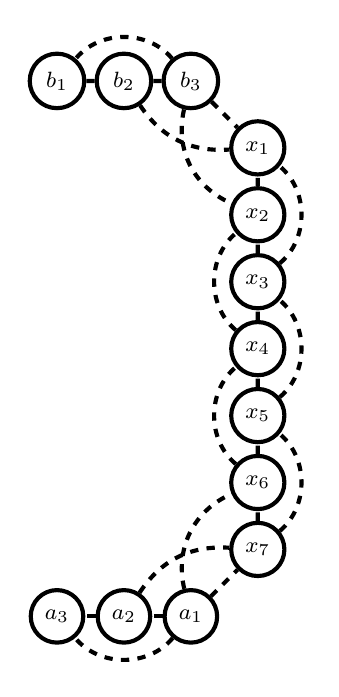
\begin{tikzpicture}[scale=0.85]
    \node[circle, draw=black, fill=white, line width=1.5pt, font=\footnotesize] (a2) at (0, 0) {$a_{3}$};
    \node[circle, draw=black, fill=white, line width=1.5pt, font=\footnotesize] (a1) at (1, 0) {$a_{2}$};
    \node[circle, draw=black, fill=white, line width=1.5pt, font=\footnotesize] (a0) at (2, 0) {$a_{1}$};

    \node[circle, draw=black, fill=white, line width=1.5pt, font=\footnotesize] (b2) at (0, 8) {$b_1$};
    \node[circle, draw=black, fill=white, line width=1.5pt, font=\footnotesize] (b1) at (1, 8) {$b_2$};
    \node[circle, draw=black, fill=white, line width=1.5pt, font=\footnotesize] (b0) at (2, 8) {$b_3$};
    
    \node[circle, draw=black, fill=white, line width=1.5pt, font=\footnotesize] (x1) at (3, 1) {$x_{7}$};
    \node[circle, draw=black, fill=white, line width=1.5pt, font=\footnotesize] (x2) at (3, 2) {$x_{6}$};
    \node[circle, draw=black, fill=white, line width=1.5pt, font=\footnotesize] (x3) at (3, 3) {$x_{5}$};
    \node[circle, draw=black, fill=white, line width=1.5pt, font=\footnotesize] (x4) at (3, 4) {$x_{4}$};
    \node[circle, draw=black, fill=white, line width=1.5pt, font=\footnotesize] (x5) at (3, 5) {$x_{3}$};
    \node[circle, draw=black, fill=white, line width=1.5pt, font=\footnotesize] (x6) at (3, 6) {$x_{2}$};
    \node[circle, draw=black, fill=white, line width=1.5pt, font=\footnotesize] (x7) at (3, 7) {$x_{1}$};
    
    \draw[line width=1.5pt, dashed] (a0) to (a1);
    \draw[line width=1.5pt, dashed] (a1) to (a2);
    \draw[line width=1.5pt, bend left=50, dashed] (a0) to (a2);

    \draw[line width=1.5pt, dashed] (b0) to (b1);
    \draw[line width=1.5pt, dashed] (b1) to (b2);
    \draw[line width=1.5pt, bend right=50, dashed] (b0) to (b2);


    \draw[line width=1.5pt, dashed] (x1) to (x2);
    \draw[line width=1.5pt, dashed] (x2) to (x3);
    \draw[line width=1.5pt, dashed] (x3) to (x4);
    \draw[line width=1.5pt, dashed] (x4) to (x5);
    \draw[line width=1.5pt, dashed] (x5) to (x6);
    \draw[line width=1.5pt, dashed] (x6) to (x7);

    \draw[line width=1.5pt, bend right=50, dashed] (x1) to (x3);
    \draw[line width=1.5pt, bend left=50, dashed] (x2) to (x4);
    \draw[line width=1.5pt, bend right=50, dashed] (x3) to (x5);
    \draw[line width=1.5pt, bend left=50, dashed] (x4) to (x6);
    \draw[line width=1.5pt, bend right=50, dashed] (x5) to (x7);

    \draw[line width=1.5pt, dashed] (a0) to (x1);
    \draw[line width=1.5pt, bend left=40, dashed] (a0) to (x2);
    \draw[line width=1.5pt, dashed, bend left=30,] (a1) to (x1);

    \draw[line width=1.5pt, dashed] (b0) to (x7);
    \draw[line width=1.5pt, bend right=40, dashed] (b0) to (x6);
    \draw[line width=1.5pt, dashed, bend right=30] (b1) to (x7);
\end{tikzpicture}
        \end{figure}
    \end{column}
\end{columns}
\end{frame}
